%% PCSJ(画像符号化シンポジウム) / IMPS(映像メディア情報シンポジウム) 用テンプレート
%% このテンプレートは「英語向け」です.
%% 日本語で論文を記述する場合は manuscript.tex を使用してください.
%
\ifdefined\pfmtname
   \documentclass[a4paper,10pt,dvipdfmx,twocolumn,english]{jsarticle}
\else
   \documentclass[a4paper,10pt,twocolumn]{article}
\fi

\usepackage{pcsjimps-e}
\usepackage[english]{ikelab-pcsjimps}

%!TEX encoding = UTF-8 Unicode
%
% 卒論 / 修論用 プリアンブル
%

%% フォント
\usepackage{lmodern}
\usepackage[scale=0.95]{tgheros}
\usepackage{textcomp}
\usepackage[scaled=0.85]{beramono}
\usepackage[T1]{fontenc}

%% パッケージ
\usepackage[cmex10]{amsmath}
\usepackage{amssymb,amsfonts,mathtools,bm}

\usepackage{graphicx,color}
\usepackage[table]{xcolor}

\usepackage[pdfborder={0 0 0}]{hyperref}
\usepackage{pxjahyper}

% caption のコロン「図4.4: キャプション」を「図4.4 キャプション」に直す
\usepackage[labelsep=quad,compatibility=false]{caption}
\usepackage[belowskip=1.2em]{subcaption}

\usepackage{cite,url,array,makecell}
\usepackage{algorithm,algorithmic}

% 数学コマンドの補完
\DeclareMathOperator*{\sinc}{sinc}
\DeclareMathOperator*{\prox}{prox}
\DeclareMathOperator*{\argmin}{argmin}
\DeclareMathOperator*{\argmax}{argmax}

% 参考文献表示スタイルを変更
\bibliographystyle{sieicej}

% 赤色を少し暗くする
\definecolor{red}{rgb}{0.75,0,0}

\makeatletter
   % アルゴリズム図キャプションの表記を「Algorithm」→「アルゴリズム」に
   \renewcommand{\ALG@name}{アルゴリズム}
\makeatother

% 修正箇所に色付けするコマンド
%
% ・ コマンド版
%   \fixed{修正箇所}
%
% ・ 環境版
%   \begin{fixedregion}
%      修正箇所
%   \end{fixedregion}
\newcommand{\fixed}[1]{#1} 
\newenvironment{fixedregion}{\ignorespaces}{\ignorespacesafterend}
% 下の 2 行をコメントアウトすることで色付けを無効化します
\renewcommand{\fixed}[1]{\textcolor{red}{#1}}
\renewenvironment{fixedregion}{\protect\leavevmode\color{red}\ignorespaces}{\ignorespacesafterend}

% 強調
\newcommand{\strong}[1]{\textcolor{red}{\textbf{#1}}}



%% 論文タイトル
\title{How to Prepare a Camera-Ready Paper for Picture Coding Symposium of Japan and Image Media Processing Symposium}

%% 著者
\author{
   % \EAuthor{著者}{この著者を表示するのに必要な横幅}
   \EAuthor{Takanori Fujisawa$^\dag$}{.3\hsize}
   \EAuthor{Masaaki Ikehara$^\dag$}{.3\hsize}
}

\affiliate{
   % \EAffiliation{英語所属名}{この所属を表示するのに必要な横幅}
   \EAffiliation{$^\dag$EEE Department, Keio University}{.9\hsize}
}

\begin{abstract}
   Put your English abstract in 100 words.
   %
This paper proposes a novel method to estimate non-integer shift of images based on least squares approximation in the phase region. Conventional methods based on Phase Only Correlation (POC) take correlation between an image and its shifted image, and then estimate the non-integer shift by fitting the model equation. The problem when estimating using POC is that the estimated peak of the fitted model equation may not match the true peak of the POC function. This causes error in non-integer shift estimation. By calculating the phase difference directly in the phase region, the proposed method allows the estimation of sub-pixel shift through least squares approximation. Also by utilizing the characteristics of natural images, the proposed method limits adoption range for least squares approximation. 
By these improvements, the proposed method achieves high accuracy, and we validate through some examples.
\end{abstract}

\begin{document}

\pagestyle{empty}

\maketitle

\thispagestyle{empty}

\section{Length and Typeset Parameters}

\begin{itemize}
   \item up to two pages including figures and tables
   \item A4 size
   \item text area width of 180mm
   \item text area height of 252mm
   \item baseline skip of 8mm
\end{itemize}

\section{Introduction}
With the recent advancement of hardware technology,
   large resolution sensors capable of taking images and videos with huge data sizes have become more common. 
To utilize these huge data, the needs for technologies like video encoding, signal processing, and object recognition have increased. 
For example to handle these huge data sized videos, encoding technologies like MPEG-2 and MPEG-4 have been introduced. 
These technologies encode videos by finding the most similar patch from the frames before. 
And to find the most similar patch, shift estimation technologies are used. 
Also, shift estimation methods are very important base technology of object recognition.
For example, when manufacturing semiconductors, precise placements of components is very important, 
and it requires very accurate shift estimation for efficient production.
Therefore, the improvements of shift estimations will have a large impact.

Majority of shift estimation methods use phase only correlation of the two input images, 
   which shows sharp peak corresponding to the shift between the images. 
The sharp peak estimated by POC shows shift on integer accuracy easily. 
Therefore, main focus of current research has been the estimation of non-integer shift. 
These include methods which use calculation in frequency domain
   \cite{balci2006subpixel,hoge2003subspace,kilthau2002full,reddy1996fft}, 
   estimation of the true peak by using model equation fitting 
   \cite{pocsubimproved,takita2003high,pocsub,dobashi2013parallel}, 
   and estimation based on Discrete Cosine Transform called DCT-SPC 
   \cite{dctspc,ito2009multiple}. 
Although some methods which use model equation to estimate the true peak of the POC may have high accuracy, 
they have possibility that the true peak and the estimated peak of the model equation don't match. 
Therefore, it can be the cause of estimation error.

In this paper, we propose a new method to estimate image shift on non-integer accuracy based on least squares method in phase region.
The proposed method estimates shift directly
    in the frequency domain by calculating the slope of the phase response which corresponds to the shift of the images.  
However, the obtained phase component includes many discontinuity, because of calculation of $\tan^{-1}$. 
These discontinuities prevents us from estimating the slope which corresponds to the shift value. 
The proposed method unwraps the phase component by subtracting the phase component of the integer shift value from the original phase component. 
This way, the proposed method obtains a smooth continuous phase component,
 which allows estimation of the slope corresponding to the decimal shift directly from phase component.
Consequently, we avoid the cause of error in the conventional POC based method without using the model equation.

\section{Conventional method}%
\label{sec:poc}%
In this section, we explain the POC based shift estimation. 
The POC takes the correlation of two images in frequency domain
   to obtain the peak which corresponds to the shift value between the images.
%
\begin{figure*}[t]
   \centering
   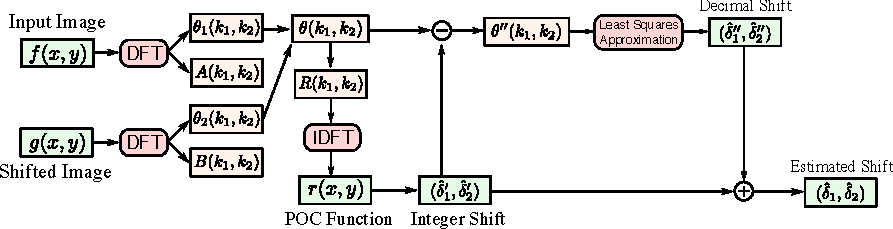
\includegraphics[width=.95\hsize]{figure/flowchart.pdf}
   \caption{Flow chart of the proposed method}
   \label{flowchart}
\end{figure*}

\subsection{Phase Only Correlation}

First we consider an image $f(x,y)$ sized $N_1 \times N_2$ and an image $g(x,y)$ 
   which is $(\delta_1,\delta_2)$ shifted image of $f(x,y)$ in parallel as they are defined below.
   \begin{align}
      x \in \{0, 1, 2,\ldots,N_1-1\} \\
      y \in \{0, 1, 2,\ldots,N_2-1\}
   \end{align}


\subsubsection{Phase Only Correlation}%
First we consider an image $f(x,y)$ sized $N_1 \times N_2$ and an image $g(x,y)$ 
   which is $(\delta_1,\delta_2)$ shifted image of $f(x,y)$ in parallel as they are defined below.
   \begin{align}
      x \in \{0, 1, 2,\ldots,N_1-1\} \\
      y \in \{0, 1, 2,\ldots,N_2-1\}
   \end{align}
Also Fourier transforms of the two images $f(x,y)$ and $g(x,y)$ are given by
   \begin{align}
      \label{F}
      F(k_1,k_2) &= \sum^{N_1-1}_{x=0}\sum^{N_2-1}_{y=0}f(x,y)e^{-j2\pi(xk_1/N_1 + yk_2/N_2)} \nonumber \\
         &= A(k_1,k_2)e^{j\theta_1(k_1,k_2)} 
   \end{align}
   \begin{align}
      G(k_1,k_2) &= \sum^{N_1-1}_{x=0}\sum^{N_2-1}_{y=0}g(x,y)e^{-j2\pi(xk_1/N_1 + yk_2/N_2)} \nonumber \\
         &= B(k_1,k_2)e^{j\theta_2(k_1,k_2)} 
      \label{G}
   \end{align}
   where $A(k_1,k_2)$ and $B(k_1,k_2)$ represent the amplitude components, 
   $e^{j\theta_i(k_1,k_2)}$ are the phase components of their images, 
   and $j$ denotes an imaginary unit.
Now, a normalized cross power spectrum $R$ is given by
   \begin{equation}
      R(k_1,k_2) = \frac {F(k_1,k_2) G^*(k_1,k_2)}{|F(k_1,k_2)  G^*(k_1,k_2)|}
   \end{equation}
   where $G^{*}(k_1,k_2)$ denotes a complex conjugate of $G(k_1,k_2)$.
Therefore $R$ can be represented as follows from (\ref{F}) and (\ref{G})
   \begin{equation}
      \label{eq_powspec}
      R(k_1,k_2) = e^{j\theta(k_1,k_2)}
   \end{equation}
   where $\theta(k_1,k_2) = \theta_1(k_1,k_2) - \theta_2(k_1,k_2)$, which is the phase difference of the two input images.
Then, the POC function $r(x, y)$ of the two images are given 
   by 2-D inverse discrete Fourier transform of $R(k_1,k_2)$ by
   \begin{equation}
      r(x,y) = \frac{1}{N_1N_2} \sum^{N_1-1}_{k_1=0}\sum^{N_2-1}_{k_2=0}R(k_1,k_2)e^{j2\pi(k_1x/N_1+k_2y/N_2)}
   \end{equation}
Fig.~\ref{POCpeak_int} shows the example of POC with peak indicating integer shift value $(\delta_1, \delta_2)$.

\begin{figure}[t]
   \centering
   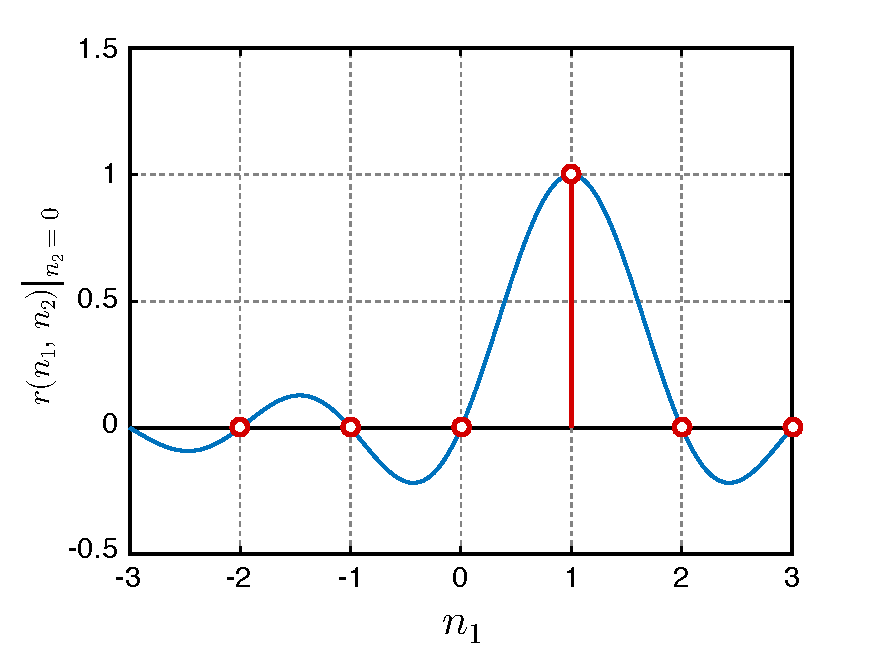
\includegraphics[width=.8\hsize]{figure/fig2.pdf}
   \caption{Example of POC function $r$ with integer shift}
   \label{POCpeak_int}
\end{figure}

\begin{figure}[t]
   \centering
   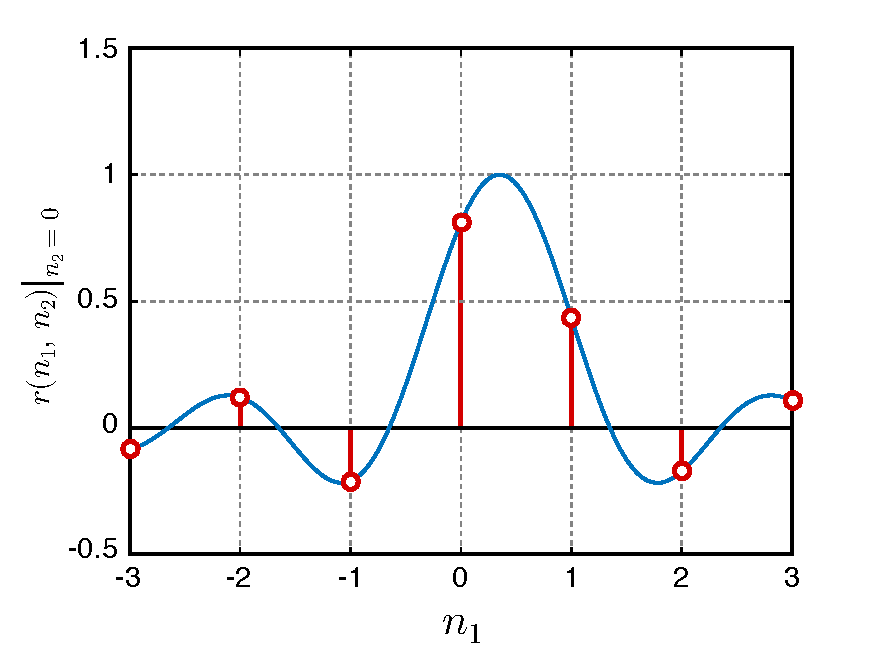
\includegraphics[width=.8\hsize]{figure/fig4.pdf}
   \caption{Example of POC function $r$ with non-integer shift and ideal model equation}
   \label{POCpeak_nonint}
\end{figure}

\subsection{Non-integer shift estimation}

The peak of the POC function $r(x,y)$ only shows the integer shift
    $(\delta^\prime_1,\delta_2^\prime)$ of the images. 
To estimate the non-integer shift of the images, 
   estimating the true peak of the POC function is necessary like in Fig.~\ref{POCpeak_nonint}. 
Conventional methods use the model equation fitting to estimate the true peak. 
   The conventional methods \cite{takita2003high,dctspc,ito2009multiple}
       uses the model equation shown as follows:
   \begin{equation}
      \label{eq:POC fitting model}
      r(x,y) \simeq \frac{1}{N_1N_2} 
         \frac{\sin{\pi(x+\delta_1)}}{\sin{\frac{\pi}{N_1}(x+\delta_1)}} 
      \frac{\sin{\pi(y+\delta_2)}}{\sin{\frac{\pi}{N_2}(y+\delta_2)}}.
   \end{equation}


\subsection{Problem with conventional method}
\label{problemofCM}
In order for the conventional methods to estimate sub-pixel shift, 
   conventional methods need to fit the model equation to the calculated POC function $r(x,y)$. 
However, it is not certain that the estimated peak 
   of the model equation matches the true peak of the POC function $r(x,y)$.
Also fitting of model equation requires multiple calculations, 
   which leads to larger computational time.
By avoiding the fitting of the model equation, 
   the proposed method estimates the shift directly from the phase components of the two images.


\section{Format Outline}

\begin{itemize}
   \item abstract of about 100 words
   \item manuscript can be either one-column or two-column.
   \item put the contact information at the bottom-right of the 
         last page. (You may want to use sample macro \verb|\simplefootnotetext|).
\end{itemize}

\section{Font Sizes}

Following font sizes are recommended.
\begin{description}
   \item[Title] 16pt (\verb|\LARGE|)
   \item[Author names] 12pt(\verb|\large|)
   \item[Affiliation and text] 10pt(\verb|\normalsize|)
\end{description}


\section{Tables and Figures}
Please be aware that your manuscript will be printed in monochrome, 
halftone dot meshing.

Figures and tables shall be placed at the top or bottom of a column wherever possible.
For \TeX floats, the placement parameter shall be either [t] or [b]. [h] shall be 
used sparingly, or not at all.
Refer to them with e.g., 
\figref{results} and \tabref{settings}.

\section{Other \LaTeXe-Specific Tips}

You may use newtx\cite{dctspc} package etc. to have more beautiful typesetting.

To show URLs, consider the use of url style file with \verb|\url{http://...}|.

You may use 
hyperref package\cite{hyperref} to 
build a PDF file that contains hyperlink information. 


\begin{table}[tb]
\caption{Encoder Settings.}
\label{tab:settings}
\centering
\begin{tabular}{c||c|c}\hline
 configuration 1 & aa & aaa\\\hline
 configuration 2 & bb & bbb\\\hline
 configuration 3 & cc & ccc\\\hline
\end{tabular}
\end{table}

\begin{figure}[tb]
   \centering
   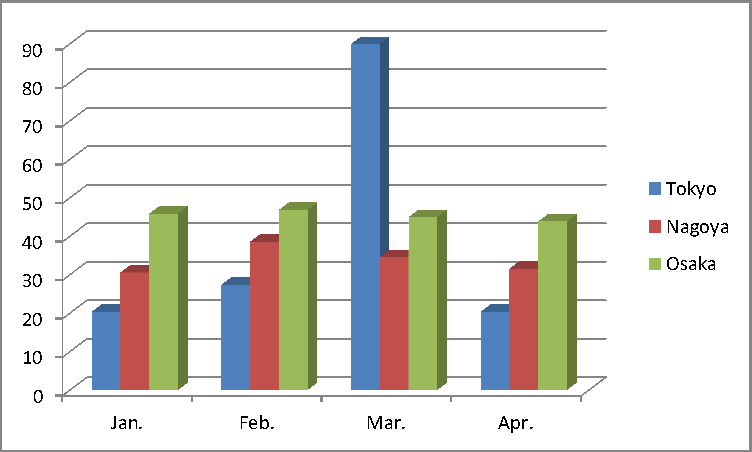
\includegraphics[width=.55\columnwidth]{figure/sample-e.pdf}\\
   \caption{Coding results.}
   \label{fig:results}
\end{figure}

\vspace{5cm}

\section{Conclusion}
2014.05.13 Initial Version\\
2015.07.15 Revised Version

\def\etal{\textit{et al.}}
\bibliographystyle{IEEETran}
\bibliography{cites}

\simplefootnotetext{
Ikehara Laboratory, EEE Department, Keio University \\ 
Kohoku-ku, Yokohama, Kanagawa, 223--8522, Japan\\
E-mail: \url{ikehara@tkhm.elec.keio.ac.jp}}

\end{document}

%#!platex
